
\section{Empirical Evidences}



\subsection{{Forecasting Comovement}}
\label{Forecasting Comovement}

	Figure \ref{mcorr50} plots stock return comovement for different levels of common ownership, measured by MFCAP.  Higher levels of common	ownership between two firms seem to be associated with stronger correlation in their stock returns. In order to study the impact of common ownership on stock return comovement, we empirically estimate the effect of lagged measures of common ownership on stock return comovement. 
	\begin{figure}[htbp]
	\centering  
	\centering
	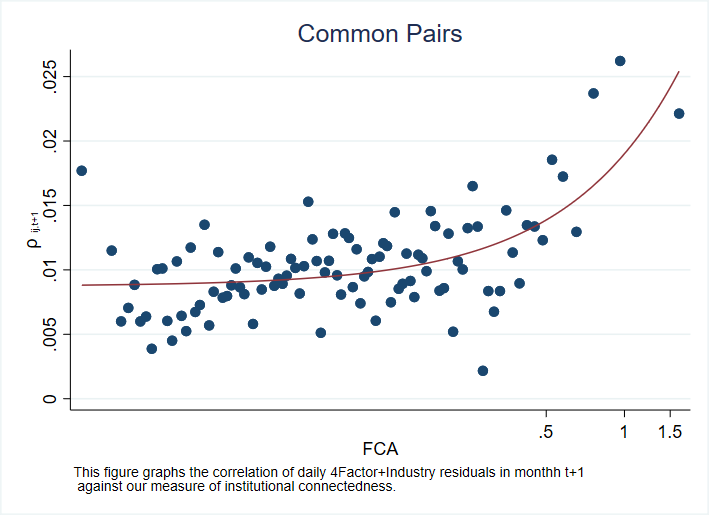
\includegraphics[width=0.7\linewidth]{"Output/mcorr50.eps"} 
	\caption{Comovement for different level of common ownership }
	\label{mcorr50}
\end{figure}
	
	We estimate a series of cross-sectional regression models in which the dependent variable is within-month realized correlation of abnormal returns of stock pairs ($\rho_{i,j,t+1}$). As explained in section \ref{comovement}, abnormal returns are the daily residuals from a model consisting of Fama-French four factors plus industry returns. The main independent variable of interest is our measure of common ownership, $\textit{MFCAP}^*_{ij,t}$. We are also interested in the effect of being part of the same business group,  $\textit{Same Group}_{ij} $, on stock return comovement.
		\begin{equation}
\begin{split}
\rho_{ij,t+1} = & \text{ 	}\beta_0 + \beta_1* \text{FCA}^*_{ij,t} + \beta_2* \text{SameGroup}_{ij} \\
 &	+\beta_3* \text{FCA}^*_{ij,t} \times \text{SameGroup}_{ij}   \\
  & + \sum_{k=1} ^{n} \alpha_k*\text{Control}_{ij,t} + \varepsilon_{ij,t+1}
\end{split}
\label{model1}
\end{equation}

	
	To mitigate the autocorrelation problem, we estimate the cross-sectional regressions each month and report the time-series average coefficients as in \cite{FamaMacBeth}. Standard errors are calculated using  \cite{newey1987hypothesis} to correct for potential autocorrelation in the time series of cross-sectional estimates for up to four lags. % \textit{ parenthesis His not necessary }($ 4(71/100)^{\frac{2}{9}} = 3.71 \sim 4 $).
	
	
The results of our Fama McBeth regressions are presented in Panel \subref{mresult2part1} of table \ref{re1}.
Column 1 reports the results of univariate regressions showing stock return comovement is significantly larger in stock pairs that have higher levels of common ownership ($ MFCAP^*_{i,j}$). 
%(\textit{we should discuss economic magnitude here, for example, going from the 25th percentile of MFCAP to 75th percentile increase comovement by X})
 In Column 2 we control for  \textit{Same Industry}, \textit{Same Size}, \textit{Same Book to Market}, and \textit{Cross-Ownership}, defined as described in Section \ref{control}. The variables \textit{Same Size} and \textit{Same Book to Market} are normalized to have a standard deviation of one and are transformed so that higher values indicate greater similarity between the two stocks in a pair. We find that our measure of common ownership, $ MFCAP^*_{i,j}$, is still significantly associated with higher stock return comovement. 
		
		
		As discussed earlier, anecdotal evidence seems to suggest common ownership in the Iranian public sector is mainly driven by business groups. The average common ownership measure, $ MFCAP^*_{i,j}$, for pairs in the same business group is five times larger than the rest.
		%we need to show this statistics somewhere.
		Hence in Column 3, we separately estimate univariate regressions of an indicator variable for whether firms in a pair are part of the same business groups on stock return comovement. We find firms that belong to the same business groups have significantly higher stock return comovement. The magnitude of this effect is economically large.
%		(\textit{add discussion for magnitude})
The estimated coefficient for \textit{SameGroup} in Column 3 is $0.036$, which is more than three times larger than the coefficient for the constant term, and is statistically significant, suggesting that return comovement in our sample is almost four times larger for firm pairs that are in the same business groups, compared to the those that are not. This result is robust to the addition of control variables as reported in Column 4. 
%According to the results, there is a significant difference in the impact of the same business groups and the common ownership
% (\textit{we can't make this claim until we discuss magnitudes earlier})
	 In Column 5, once we include both our measure of common ownership, $\textit{MFCAP}^*_{i,j}$, and \textit{Same Group} indicator in our regression model, the coefficient estimate for  \textit{Same Group} remains statistically significant and very similar in magniture compared to that in Column 4. However, the coefficent estimate on common ownership measure, $\textit{MFCAP}$, is no longer significant. This suggests that common ownership affects stock return comovement among our sample firms mostly through business group affiliations. It is also worth noting that firms in the same industry have siginificantly higher stock return comovement, as is the case for firms closer in size and book-to-market. This is in spite of
	 the fact that we already account for industry return, size and book-to-market in measuring daily residuals from equation 2. 
	  In the last column, we control for additional pair level fixed effects based on the size of the firms in a pair. Pairs are categorized into large or small if both firms are large or small. If one firm in a pair is large and the other is small, we categorize the pair as hybrid. Our results are robust to the addition of pair type fixed effects.
	  %\cite{AntonPolk} restrict their analysis to only large firms.
	 %why they do that, why we dont, and what happens if we do?.
	 

	
	
	
	In panel \subref{mresult2part2}, we examine the interaction effect of common ownership and business groups on return comovement. In Column 1, we restrict our sample only to pairs that are in the same business groups. The coefficient estimate on common ownership measure, $\textit{MFCAP}$, remains positive and highly significant. This suggest that variations in common ownership among firms in the same business group significantly impact their respective stock return comovement. In Column 2, however, we restrict our sample to firm pairs that are either not part of the same business group or do not belong to any business groups. The coefficient estimate on $\textit{MFCAP}$ here is both economically small and statistically insignificant, suggesting that measure of common ownership does not seem to be associated with return comovement among firm pairs that are not affiliated with the same business groups. As described before, this is likely due to the fact that common ownership in Iran's public firms is mostly driven by business groups, hence \textit{Same Group} indicator largely acts as a proxy for common ownership as well. Using the full sample in Column 3, we estimate our regression model by including both $\textit{MFCAP}$ and \textit{Same Group} as well as their interaction term.
	
	 It provides evidence that common ownership only matters for the pairs in the same business groups.
	Now for the main analysis, we include the interaction of \textit{Same Group} and $\text{MFCA}^*_{ij,t}$. We include the business group fixed effects to capture the group's characteristics for the last column. In these specifications, the economic effect of \textit{Same Group} is not significant anymore, which cannot be reliable due to the high correlation of interaction term with \textit{Same Group}($\rho = 0.75$). These results aver that $\text{MFCA}^*_{ij,t}$ has a larger effect for the pairs in the same business group. It puts forward that the \textit{Same Group}  affects comovement through indirect common ownership, which arises due to the same ultimate owner. 
	
	
	
	
		\captionsetup[subtable]{labelformat=parens,font=small}
			\renewcommand{\thesubtable}{\Alph{subtable}}
\newgeometry{top=20mm, bottom=30mm}
{\begin{table}[p]
		\centering
		\centerfloat
		\caption{Connected Comovement\\ \small
		This table reports \cite{FamaMacBeth} estimates of monthly cross-sectional regressions forecasting the correlation of daily \cite{fama1993differences}–\cite{Carhart4Factor} plus industry residuals in month t + 1 for the sample of stocks defined in Table \ref{st1}. The independent variables are updated monthly include our measure of institutional connectedness, the number of equal percents held block-holder, $\text{MFCA}^*_{ij,t}$, and a series of controls at time t. We measure the negative of the absolute value of the difference in size and book-to-market ratio (BE/ME) percentile ranking across the two stocks in the pair (SameSize, and SameBM, respectively). All independent variables, excluding dummy variables, are then rank-transformed and normalized to have a unit standard deviation. We calculate \cite{newey1987hypothesis} standard errors (four lags) of the \cite{FamaMacBeth} estimates that take into account autocorrelation in the cross-sectional slopes. We report the associated t-statistics in parentheses.
		We report estimates of regressions using variables to investigate the effect of common ownership and business group in Panel \subref{mresult2part1}. Panel \subref{mresult2part2} shows the estimation result for investigating the effect of common ownership in the business groups. }
		\label{re1}
		\subcaption{The main analysis}
		\label{mresult2part1}
		\resizebox{0.9\textwidth}{!}{
				{{
\def\sym#1{\ifmmode^{#1}\else\(^{#1}\)\fi}
\begin{tabular}{l*{6}{c}}
\hline\hline
                    &\multicolumn{6}{c}{Dependent Variable:  Future Pairs's Comovement}                                                                 \\\cmidrule(lr){2-7}
                    &\multicolumn{1}{c}{(1)}         &\multicolumn{1}{c}{(2)}         &\multicolumn{1}{c}{(3)}         &\multicolumn{1}{c}{(4)}         &\multicolumn{1}{c}{(5)}         &\multicolumn{1}{c}{(6)}         \\
\hline
$ \text{MFCAP*} $   &     0.00600\sym{***}&     0.00328\sym{***}&                     &                     &     0.00104         &    0.000929         \\
                    &      (8.10)         &      (4.87)         &                     &                     &      (1.68)         &      (1.53)         \\
[1em]
SameGroup           &                     &                     &      0.0358\sym{***}&      0.0254\sym{***}&      0.0242\sym{***}&      0.0219\sym{***}\\
                    &                     &                     &      (9.99)         &      (8.45)         &      (8.21)         &      (7.02)         \\
[1em]
SameIndustry        &                     &      0.0267\sym{***}&                     &      0.0216\sym{***}&      0.0212\sym{***}&      0.0215\sym{***}\\
                    &                     &      (7.39)         &                     &      (6.81)         &      (6.72)         &      (6.80)         \\
[1em]
SameBM              &                     &      0.0224\sym{***}&                     &      0.0213\sym{***}&      0.0214\sym{***}&      0.0199\sym{***}\\
                    &                     &      (6.41)         &                     &      (6.09)         &      (6.16)         &      (5.77)         \\
[1em]
SameSize            &                     &      0.0123\sym{**} &                     &      0.0143\sym{***}&      0.0138\sym{***}&      0.0254\sym{***}\\
                    &                     &      (3.24)         &                     &      (3.85)         &      (3.71)         &      (5.56)         \\
[1em]
CrossOwnership      &                     &      0.0600\sym{***}&                     &      0.0300\sym{*}  &      0.0316\sym{*}  &      0.0377\sym{**} \\
                    &                     &      (5.50)         &                     &      (2.36)         &      (2.48)         &      (2.93)         \\
[1em]
Constant            &      0.0142\sym{***}&      0.0204\sym{***}&      0.0103\sym{***}&      0.0187\sym{***}&      0.0188\sym{***}&      0.0280\sym{***}\\
                    &     (12.80)         &      (8.91)         &      (9.42)         &      (7.99)         &      (8.04)         &      (9.43)         \\
\hline
PairType Control    &          No         &          No         &          No         &          No         &          No         &         Yes         \\
Observations        &      389591         &      389591         &      389591         &      389591         &      389591         &      389591         \\
\hline\hline  \end{tabular}}
}
		}
		\bigskip
		\subcaption{Common Ownership and Business Group}
		\label{mresult2part2}
		\resizebox{0.9\textwidth}{!}{
					
						{{
\def\sym#1{\ifmmode^{#1}\else\(^{#1}\)\fi}
\begin{tabular}{l*{4}{c}}
\hline\hline
                &\multicolumn{4}{c}{Dependent Variable: Future Pairs's co-movement'}        \\\cmidrule(lr){2-5}
                &\multicolumn{1}{c}{(1)}         &\multicolumn{1}{c}{(2)}         &\multicolumn{1}{c}{(3)}         &\multicolumn{1}{c}{(4)}         \\
\hline
$ \text{MFCAP*} $&  0.00944\sym{***}& 0.000397         & 0.000377         &-0.0000113         \\
                &   (7.24)         &   (0.68)         &   (0.65)         &  (-0.02)         \\
[1em]
Same Group      &                  &                  &  0.00624\sym{**} &  0.00549\sym{*}  \\
                &                  &                  &   (2.81)         &   (2.27)         \\
[1em]
 $ (\text{MFCAP}^*) \times {\text{SameGroup} }  $ &                  &                  &  0.00992\sym{***}&   0.0107\sym{***}\\
                &                  &                  &   (6.49)         &   (6.97)         \\
\hline
Observations    &    58337         &  1607659         &  1665996         &  1665996         \\
Sub-sample      &SameGroup         &   Others         &      All         &      All         \\
Group Effect    &       No         &       No         &       No         &      Yes         \\
Controls        &      Yes         &      Yes         &      Yes         &      Yes         \\
$ R^2 $         &   0.0112         & 0.000577         & 0.000898         &  0.00575         \\
\hline\hline
\multicolumn{5}{l}{\footnotesize \textit{t} statistics in parentheses}\\
\multicolumn{5}{l}{\footnotesize \sym{*} \(p<0.05\), \sym{**} \(p<0.01\), \sym{***} \(p<0.001\)}\\
\end{tabular}
}
}
					
				}
		
\end{table}}
\restoregeometry
%{\begin{table}[p]
%		\centering
%		\caption{Connected Comovement}
%		\label{mresult2part2}
%		\resizebox{1\textwidth}{!}{
%			
%				{{
\def\sym#1{\ifmmode^{#1}\else\(^{#1}\)\fi}
\begin{tabular}{l*{4}{c}}
\hline\hline
                &\multicolumn{4}{c}{Dependent Variable: Future Pairs's co-movement'}        \\\cmidrule(lr){2-5}
                &\multicolumn{1}{c}{(1)}         &\multicolumn{1}{c}{(2)}         &\multicolumn{1}{c}{(3)}         &\multicolumn{1}{c}{(4)}         \\
\hline
$ \text{MFCAP*} $&  0.00944\sym{***}& 0.000397         & 0.000377         &-0.0000113         \\
                &   (7.24)         &   (0.68)         &   (0.65)         &  (-0.02)         \\
[1em]
Same Group      &                  &                  &  0.00624\sym{**} &  0.00549\sym{*}  \\
                &                  &                  &   (2.81)         &   (2.27)         \\
[1em]
 $ (\text{MFCAP}^*) \times {\text{SameGroup} }  $ &                  &                  &  0.00992\sym{***}&   0.0107\sym{***}\\
                &                  &                  &   (6.49)         &   (6.97)         \\
\hline
Observations    &    58337         &  1607659         &  1665996         &  1665996         \\
Sub-sample      &SameGroup         &   Others         &      All         &      All         \\
Group Effect    &       No         &       No         &       No         &      Yes         \\
Controls        &      Yes         &      Yes         &      Yes         &      Yes         \\
$ R^2 $         &   0.0112         & 0.000577         & 0.000898         &  0.00575         \\
\hline\hline
\multicolumn{5}{l}{\footnotesize \textit{t} statistics in parentheses}\\
\multicolumn{5}{l}{\footnotesize \sym{*} \(p<0.05\), \sym{**} \(p<0.01\), \sym{***} \(p<0.001\)}\\
\end{tabular}
}
}
%			
%		}
%\end{table}}


		\FloatBarrier

		
		
		
		
		
		
		
		
		\subsection{{High level of common ownership}}
		
In line with the previous estimations, figure \ref{Qmcorr5lrd} provides that a higher level of common ownership affects more on the firms' comovement. As shown in panel  \subref{measureResults} table \ref{st2}, pairs in the same business group have a higher level of common ownership than others. So, the previous results could be driven by a high level of common ownership. For detailed analysis, we define a dummy variable for the higher level of common ownership, which we define as the pairs with $\text{MFCAP}_{ij,t}$ in the fourth quarter in each period. Figure \ref{Qmcorr5subsample} shows the relation between future comovement and current measurement of common ownership for that pairs. As shown in the right panel, in line with the last explanation, common ownership only affects the pairs in the same group, and common ownership without the same group will not affect pairs' comovement, although for a high level of common ownership.
			
			
			\begin{figure}[htbp]
				\centering  
				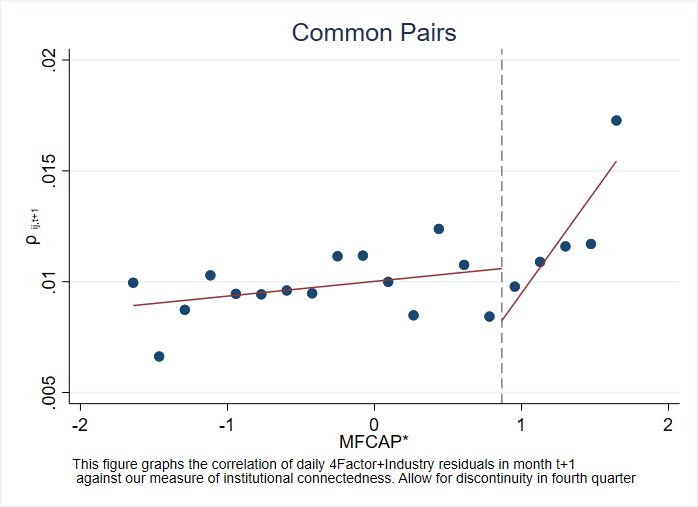
\includegraphics[width=0.65\linewidth]{"Output/Qmcorr5lrd.eps"}
				\caption{ Comovement for different level of common ownership}
				\label{Qmcorr5lrd}
			\end{figure}
			
			
						\begin{figure}[htbp]
							\centerfloat
							\resizebox{1.3\textwidth}{!}{
							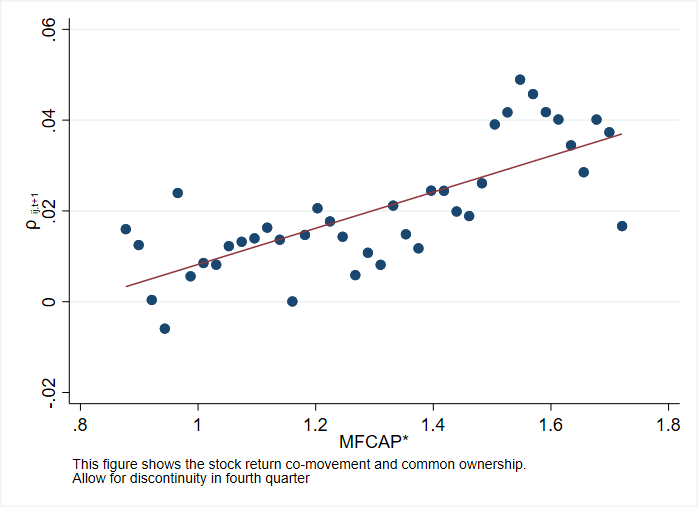
\includegraphics[width=0.55\linewidth]{"Output/Qmcorr5subsample.eps"}
							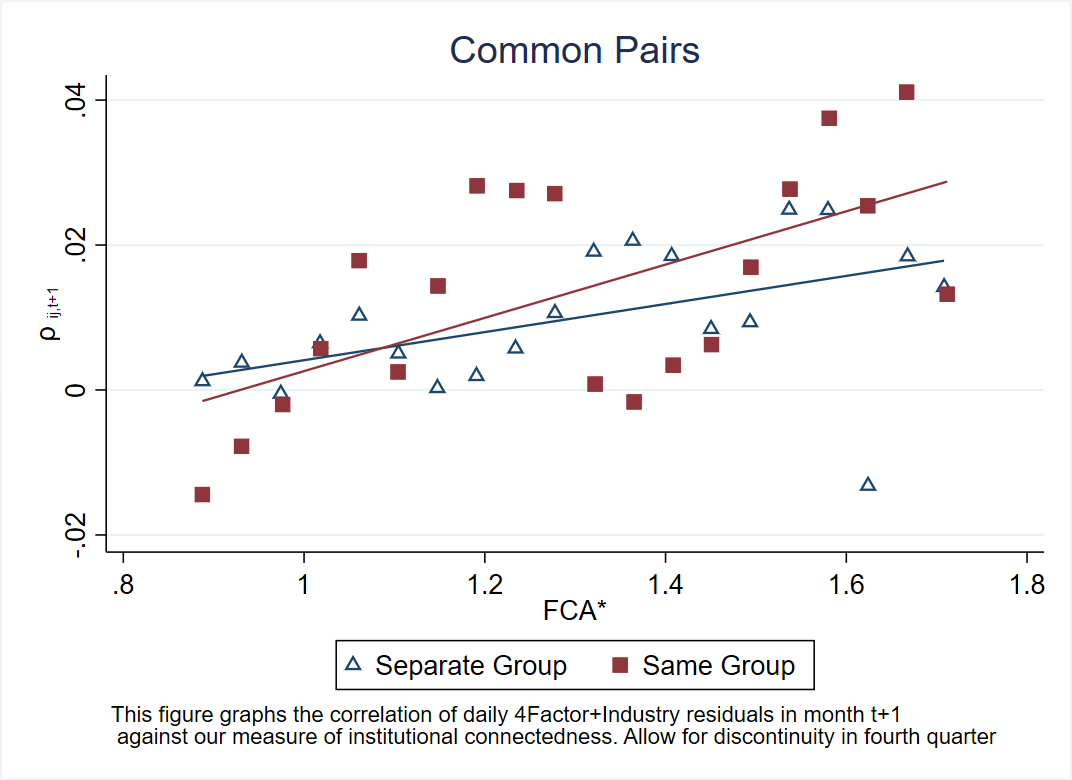
\includegraphics[width=0.55\linewidth]{"Output/Qmcorr5lrdbgsubsample.eps"}}
%							\label{Qmcorr5subsamplebg}
							\caption{Comovement for different level of common ownership for pairs in the fourth quarter}
								\label{Qmcorr5subsample}
						\end{figure}
%			\begin{figure}[htbp]
%				\centering  
%				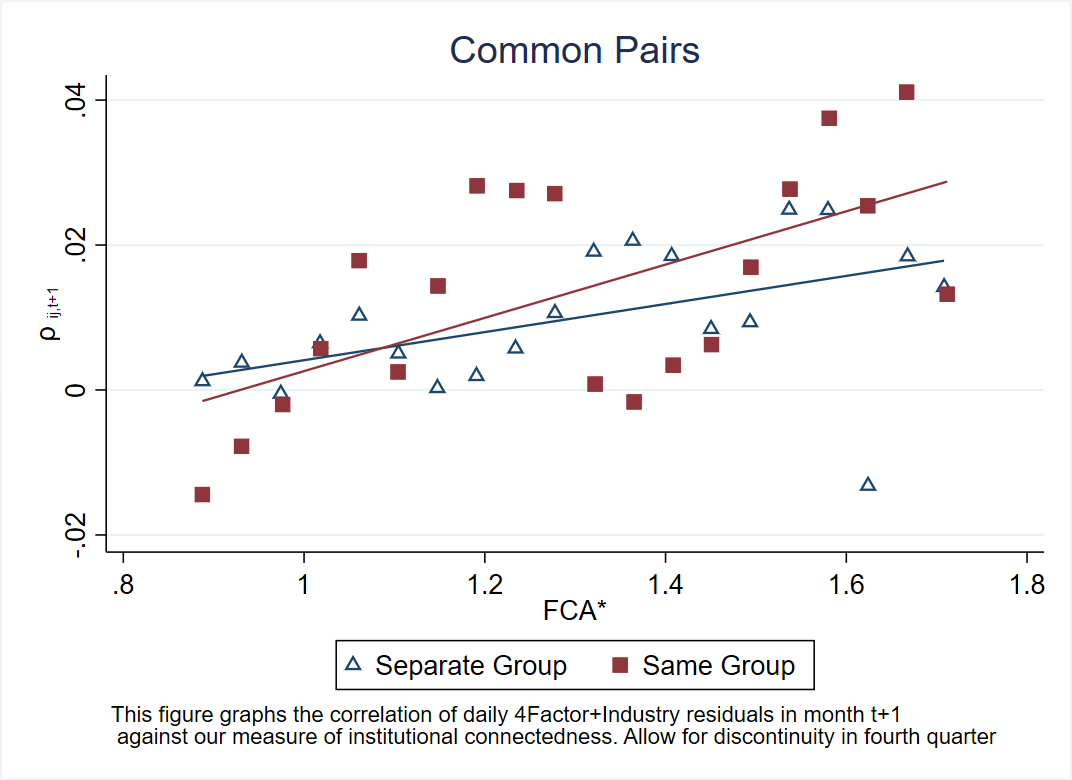
\includegraphics[width=0.65\linewidth]{"Output/Qmcorr5lrdbgsubsample.eps"}
%				\caption{Comovement for different level of common ownership for pairs in the fourth quarter}
%				\label{Qmcorr5subsamplebg}
%			\end{figure}
			
			
	
	We estimate the equation \ref{model1} with the same methodology in section \ref{Forecasting Comovement}  for the sub-sample of a high level of common ownership. Panel \subref{QTimemresult2subsample} of table \ref{re2}  reports estimations results. As expected, firms in the same business group have a high statistical and economically significant effect on forecasting future comovements. Columns three to seven confirm our prior explanations for the importance of business groups compared to common ownership in pairs with a higher level of common ownership. Pairs in the fourth quarter may have different characteristics that affect our results. In table \ref{QarterSummary}, we summarized our control variables which shows that pairs' attributes do not look significantly different than other pairs except the presence of the pairs in the same group, which we want to examine this feature.
	
%			{\begin{table}[htbp]
%					\centering
%					\caption{High level of common ownership\\ \small
%					This table reports \cite{FamaMacBeth} estimates of monthly cross-sectional regressions forecasting the correlation of daily \cite{fama1993differences}–\cite{Carhart4Factor} plus industry residuals in month t + 1 for the pairs with the high level of common ownership. This means that our estimation is limited to the subsample of stocks defined in Table \ref{t2-2} with common ownership, which is in the fourth quarter of each period. The independent variables are updated monthly include our measure of institutional connectedness, the number of equal percents held block-holder, $\text{MFCAP}^*_{ij,t}$, and a series of controls at time t. We measure the negative of the absolute value of the difference in size and book-to-market ratio (BE/ME) percentile ranking across the two stocks in the pair (SameSize, and SameBM, respectively). All independent variables, excluding dummy variables, are then rank-transformed and normalized to have a unit standard deviation. We calculate \cite{newey1987hypothesis} standard errors (four lags) of the \cite{FamaMacBeth} estimates that take into account autocorrelation in the cross-sectional slopes. We report the associated t-statistics in parentheses. Controls not shown here are reported in the Internet Appendix.}
%					\label{QTimemresult2subsample}
%					{
%						\resizebox{\textwidth}{!}{
%						{
\def\sym#1{\ifmmode^{#1}\else\(^{#1}\)\fi}
\begin{tabular}{l*{7}{c}}
\hline\hline
                &\multicolumn{7}{c}{Dependent Variable:  Future Pairs's Comovement}                                                                  \\\cmidrule(lr){2-8}
                &\multicolumn{1}{c}{(1)}         &\multicolumn{1}{c}{(2)}         &\multicolumn{1}{c}{(3)}         &\multicolumn{1}{c}{(4)}         &\multicolumn{1}{c}{(5)}         &\multicolumn{1}{c}{(6)}         &\multicolumn{1}{c}{(7)}         \\
\hline
SameGroup       &   0.0254\sym{***}&                  &   0.0249\sym{***}&                  &                  &  0.00477         &  0.00252         \\
                &   (8.45)         &                  &   (8.21)         &                  &                  &   (1.32)         &   (0.66)         \\
[1em]
$ (\text{MFCAP} > \text{Larger than 75th Percentile}) $ &                  &  0.00660\sym{***}& 0.000777         &   0.0230\sym{***}& -0.00258\sym{*}  & -0.00157         &-0.000513         \\
                &                  &   (5.48)         &   (0.73)         &   (7.09)         &  (-2.00)         &  (-1.29)         &  (-0.46)         \\
[1em]
 $ (\text{MFCAP} > Q3[\text{MFCAP}]) \times {\text{SameGroup}} $ &                  &                  &                  &                  &                  &   0.0248\sym{***}&   0.0237\sym{***}\\
                &                  &                  &                  &                  &                  &   (7.24)         &   (7.34)         \\
\hline
Sub-sample      &      All         &      All         &      All         &SameGroup         &   Others         &      All         &      All         \\
Controls        &      Yes         &      Yes         &      Yes         &      Yes         &      Yes         &      Yes         &      Yes         \\
Business Group FE&       No         &       No         &       No         &       No         &       No         &       No         &      Yes         \\
Observations    &   389591         &   389591         &   389591         &    47076         &   342515         &   389591         &   389591         \\
\hline\hline
\multicolumn{8}{l}{\footnotesize \textit{t} statistics in parentheses}\\
\multicolumn{8}{l}{\footnotesize \sym{*} \(p<0.05\), \sym{**} \(p<0.01\), \sym{***} \(p<0.001\)}\\
\end{tabular}
}

%						}
%					}
%			\end{table}}
			
%			\begin{figure}[htbp]
%				\centering  
%				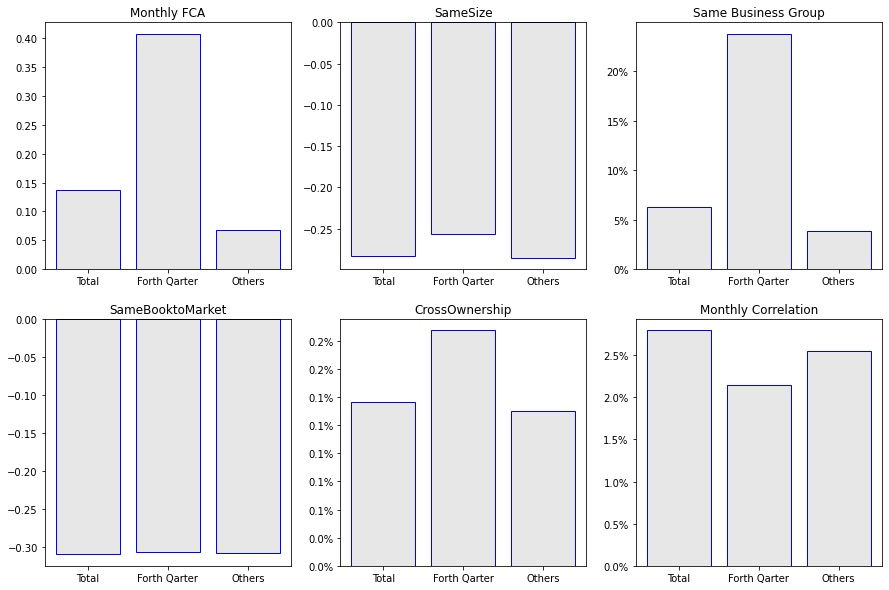
\includegraphics[width=1\linewidth]{"Output/QarterSummary.eps"}
%				\caption{Pairs' characteristics for the pairs with high level of common ownership}
%				\label{QarterSummary}
%			\end{figure}
		

				
				
				\FloatBarrier
				
				\subsection{All Pairs}
				
We restrict our investigations to firms with at least one common owner in the former analyses. By this analysis, we cannot separate the effect of the business group and common ownership; both of them can affect comovement. Furthermore, this restriction limits our result to commonly held firms, but if belonging to the same business group can increase stocks' comovement, it would affect all the firms in the same business groups. 	So, we extend our investigations by constructing all the pairs in the market to separate the effect of direct common ownership and business group and solve the mentioned problems. 
	
	For this purpose, we include stocks in one pair if they have at least two months in common. By this definition, we do not restrict our investigation to commonly held stocks and set $\text{MFCA}_{ij,t}$ to zero for a pair without any common owner. Controls are defined as before, and we use equation \ref{model1} by the same methodology as used in section \ref{Forecasting Comovement}.
	
	Panel \subref{AllPairs} table \ref{re2} reports results of estimations. These results suggest that pairs in the same group comove more than stocks not in the same group. In addition, pairs with common ownership common do not comove greater than others. In column three, we use variables of common ownership and the same business group together. Results supported our previous explanation of table \ref{re1}. The \textit{Same Group} is critical for forecasting future comovement, and common ownership matters for the pairs in the same business group.
					
%					{\begin{table}[htbp]
%							%	\centering
%							
%							\caption{Non-connected Comovement\\ \small
%							This table reports \cite{FamaMacBeth} estimates of monthly cross-sectional regressions forecasting the correlation of daily \cite{fama1993differences}–\cite{Carhart4Factor} plus industry residuals in month t + 1 for all the pairs in the market. This means that our estimation is extended to the pairs with stocks that have at least two months in common and set $\text{MFCA}_{ij,t}$ to zero for a pair without any common owner. The independent variables are updated monthly include our measure of institutional connectedness, the number of equal percents held block-holder, $\text{MFCA}^*_{ij,t}$, and a series of controls at time t. We measure the negative of the absolute value of the difference in size and book-to-market ratio (BE/ME) percentile ranking across the two stocks in the pair (SameSize, and SameBM, respectively). All independent variables, excluding dummy variables, are rank-transformed and normalized to have a unit standard deviation. We calculate \cite{newey1987hypothesis} standard errors (four lags) of the \cite{FamaMacBeth} estimates that take into account autocorrelation in the cross-sectional slopes. We report the associated t-statistics in parentheses. Controls not shown here are reported in the Internet Appendix.}			
%							\label{AllPairs}				
%							\resizebox{1\textwidth}{!}{
%									{	{
\def\sym#1{\ifmmode^{#1}\else\(^{#1}\)\fi}
\begin{tabular}{l*{7}{c}}
\hline\hline
                &\multicolumn{7}{c}{Dependent Variable: Future Pairs' co-movement}                                                                   \\\cmidrule(lr){2-8}
                &\multicolumn{1}{c}{(1)}         &\multicolumn{1}{c}{(2)}         &\multicolumn{1}{c}{(3)}         &\multicolumn{1}{c}{(4)}         &\multicolumn{1}{c}{(5)}         &\multicolumn{1}{c}{(6)}         &\multicolumn{1}{c}{(7)}         \\
\hline
SameGroup       &   0.0156\sym{***}&                  &   0.0158\sym{***}&                  &                  &   0.0138\sym{***}&   0.0131\sym{***}\\
                &   (9.84)         &                  &  (10.22)         &                  &                  &   (8.27)         &   (7.68)         \\
[1em]
$ \text{MFCAP*}  $&                  &-0.0000723         &-0.000277         &  0.00169         &-0.000322\sym{*}  &-0.000390\sym{**} &-0.000427\sym{*}  \\
                &                  &  (-0.44)         &  (-1.80)         &   (1.42)         &  (-2.19)         &  (-2.70)         &  (-2.29)         \\
[1em]
 $ (\text{MFCAP}^*) \times {\text{SameGroup} }  $ &                  &                  &                  &                  &                  &  0.00313\sym{**} &  0.00364\sym{**} \\
                &                  &                  &                  &                  &                  &   (2.80)         &   (3.34)         \\
\hline
Controls        &      Yes         &      Yes         &      Yes         &      Yes         &      Yes         &      Yes         &      Yes         \\
Sub-Sample      &    Total         &    Total         &    Total         &SameGroups         &   Others         &    Total         &    Total         \\
Business Group FE&       No         &       No         &       No         &       No         &       No         &       No         &      Yes         \\
Observations    &  6018646         &  6018646         &  6018646         &   114526         &  5904120         &  6018646         &  6018646         \\
\hline\hline
\multicolumn{8}{l}{\footnotesize \textit{t} statistics in parentheses}\\
\multicolumn{8}{l}{\footnotesize \sym{*} \(p<0.05\), \sym{**} \(p<0.01\), \sym{***} \(p<0.001\)}\\
\end{tabular}
}

%									}
%							}
%					\end{table}}
					
				
					
					
%					
%					In conclusion , these results show that same business group is more important than common ownership. In fact, when we talk about the presence of two stocks in the same business group, we talk about a high level of invisible common ownership between two stocks that we cannot measure that by mutual stockholders.
					
{\begin{table}[htbp]
		\centerfloat
			\caption{Connected Comovement\\ \small
				Panel \subref{QTimemresult2subsample} represents the estimates of monthly cross-sectional regressions forecasting the comovement for the high level of common ownership. This means that our estimation is limited to the subsample of stocks defined in Table \ref{st1} with common ownership, which is in the fourth quarter of each period. Panel \subref{AllPairs} shows the results for the estimation of that feature for all the pairs in the market, which means that the pairs with stocks that have at least two months in common and set $\text{MFCA}_{ij,t}$ to zero for a pair without any common owner. Other methods and definitions of variables are as the table \ref{re1}.  }
				\label{re2}
		\subcaption{High level of Common Ownership}
						\label{QTimemresult2subsample}
						{
							\resizebox{\textwidth}{!}{
							{
\def\sym#1{\ifmmode^{#1}\else\(^{#1}\)\fi}
\begin{tabular}{l*{7}{c}}
\hline\hline
                &\multicolumn{7}{c}{Dependent Variable:  Future Pairs's Comovement}                                                                  \\\cmidrule(lr){2-8}
                &\multicolumn{1}{c}{(1)}         &\multicolumn{1}{c}{(2)}         &\multicolumn{1}{c}{(3)}         &\multicolumn{1}{c}{(4)}         &\multicolumn{1}{c}{(5)}         &\multicolumn{1}{c}{(6)}         &\multicolumn{1}{c}{(7)}         \\
\hline
SameGroup       &   0.0254\sym{***}&                  &   0.0249\sym{***}&                  &                  &  0.00477         &  0.00252         \\
                &   (8.45)         &                  &   (8.21)         &                  &                  &   (1.32)         &   (0.66)         \\
[1em]
$ (\text{MFCAP} > \text{Larger than 75th Percentile}) $ &                  &  0.00660\sym{***}& 0.000777         &   0.0230\sym{***}& -0.00258\sym{*}  & -0.00157         &-0.000513         \\
                &                  &   (5.48)         &   (0.73)         &   (7.09)         &  (-2.00)         &  (-1.29)         &  (-0.46)         \\
[1em]
 $ (\text{MFCAP} > Q3[\text{MFCAP}]) \times {\text{SameGroup}} $ &                  &                  &                  &                  &                  &   0.0248\sym{***}&   0.0237\sym{***}\\
                &                  &                  &                  &                  &                  &   (7.24)         &   (7.34)         \\
\hline
Sub-sample      &      All         &      All         &      All         &SameGroup         &   Others         &      All         &      All         \\
Controls        &      Yes         &      Yes         &      Yes         &      Yes         &      Yes         &      Yes         &      Yes         \\
Business Group FE&       No         &       No         &       No         &       No         &       No         &       No         &      Yes         \\
Observations    &   389591         &   389591         &   389591         &    47076         &   342515         &   389591         &   389591         \\
\hline\hline
\multicolumn{8}{l}{\footnotesize \textit{t} statistics in parentheses}\\
\multicolumn{8}{l}{\footnotesize \sym{*} \(p<0.05\), \sym{**} \(p<0.01\), \sym{***} \(p<0.001\)}\\
\end{tabular}
}

							}
						}
						\bigskip
						\subcaption{All the Pairs}
\label{AllPairs}				
		\resizebox{\textwidth}{!}{
				{	{
\def\sym#1{\ifmmode^{#1}\else\(^{#1}\)\fi}
\begin{tabular}{l*{7}{c}}
\hline\hline
                &\multicolumn{7}{c}{Dependent Variable: Future Pairs' co-movement}                                                                   \\\cmidrule(lr){2-8}
                &\multicolumn{1}{c}{(1)}         &\multicolumn{1}{c}{(2)}         &\multicolumn{1}{c}{(3)}         &\multicolumn{1}{c}{(4)}         &\multicolumn{1}{c}{(5)}         &\multicolumn{1}{c}{(6)}         &\multicolumn{1}{c}{(7)}         \\
\hline
SameGroup       &   0.0156\sym{***}&                  &   0.0158\sym{***}&                  &                  &   0.0138\sym{***}&   0.0131\sym{***}\\
                &   (9.84)         &                  &  (10.22)         &                  &                  &   (8.27)         &   (7.68)         \\
[1em]
$ \text{MFCAP*}  $&                  &-0.0000723         &-0.000277         &  0.00169         &-0.000322\sym{*}  &-0.000390\sym{**} &-0.000427\sym{*}  \\
                &                  &  (-0.44)         &  (-1.80)         &   (1.42)         &  (-2.19)         &  (-2.70)         &  (-2.29)         \\
[1em]
 $ (\text{MFCAP}^*) \times {\text{SameGroup} }  $ &                  &                  &                  &                  &                  &  0.00313\sym{**} &  0.00364\sym{**} \\
                &                  &                  &                  &                  &                  &   (2.80)         &   (3.34)         \\
\hline
Controls        &      Yes         &      Yes         &      Yes         &      Yes         &      Yes         &      Yes         &      Yes         \\
Sub-Sample      &    Total         &    Total         &    Total         &SameGroups         &   Others         &    Total         &    Total         \\
Business Group FE&       No         &       No         &       No         &       No         &       No         &       No         &      Yes         \\
Observations    &  6018646         &  6018646         &  6018646         &   114526         &  5904120         &  6018646         &  6018646         \\
\hline\hline
\multicolumn{8}{l}{\footnotesize \textit{t} statistics in parentheses}\\
\multicolumn{8}{l}{\footnotesize \sym{*} \(p<0.05\), \sym{**} \(p<0.01\), \sym{***} \(p<0.001\)}\\
\end{tabular}
}

				}
		}		
		
	\end{table}}


					
					\FloatBarrier

	\captionsetup[subtable]{labelformat=empty}
